% 1992 年上海卷第 26 题：双曲线 C 的上半支顶点 A，直线 y=-x 与 C 交于点 P，以 A 为焦点、M 为顶点的开口向下抛物线过 P
% 依固定扫描页重绘，只画拓扑与标号，不按比例
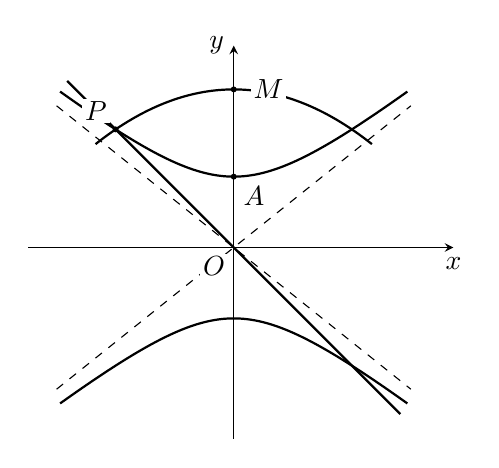
\begin{tikzpicture}[>=stealth,scale=0.9,line join=round]
  % 坐标轴
  \draw[->] (-2.9,0)--(3.1,0) node[below] {$x$};
  \draw[->] (0,-2.7)--(0,2.85) node[left] {$y$};
  % 渐近线 y=±0.8x
  \draw[dashed] (-2.5,-2.0)--(2.5,2.0);
  \draw[dashed] (-2.5,2.0)--(2.5,-2.0);
  % 双曲线 y^2 - x^2/1.5625 = 1
  \draw[thick,domain=-2.45:2.45,samples=90] plot (\x,{sqrt(1+\x*\x/1.5625)});
  \draw[thick,domain=-2.45:2.45,samples=90] plot (\x,{-sqrt(1+\x*\x/1.5625)});
  % 直线 y=-x
  \draw[thick] (-2.35,2.35)--(2.35,-2.35);
  % 抛物线 x^2 = -4.924(y-2.231)
  \draw[thick,domain=-1.95:1.95,samples=70] plot (\x,{2.231-0.2031*\x*\x});
  % 关键点
  \coordinate (P) at (-1.667,1.667);
  \coordinate (A) at (0,1);
  \coordinate (M) at (0,2.231);
  \fill (P) circle (1.2pt) node[fill=white,inner sep=1pt,above left=2pt] {$P$};
  \fill (A) circle (1.2pt) node[below right] {$A$};
  \fill (M) circle (1.2pt) node[fill=white,inner sep=1pt,right=6pt] {$M$};
  \node[fill=white,inner sep=1pt,below left=2pt] at (0,0) {$O$};
\end{tikzpicture}
